\chapter{Konzeption}\label{chapter:Konzeption}
In diesem Kapitel werden zunächst Kriterien definiert, die das Anwendungssystem im Rahmen dieser Abschlussarbeit erfüllen soll. Hierbei wird auf die Zielsetzung geachtet und Anwendungsfälle, sogenannte \textit{Use Cases}, entwickelt, die ein Anwender mit der prototypischen Implementierung bestreiten können soll. Des Weiteren wird der Systementwurf genauer betrachtet. Dazu zählen insbesondere das Zusammenwirken der einzelnen Komponenten, welche Schichten abstrahiert werden und wie der Informationsfluss in den einzelnen Komponenten ist.
\section{Spezifikation}
Bei der zu entwickelnden Software handelt es sich um ein \textit{User Interface}, dass den Anwender dazu befähigt einen Roboter mit Hilfe der Gesten- und Stimmenerkennung der \textit{Microsoft HoloLens} über das Netzwerk fernzusteuern. Für die Verwendung wird ein Roboter, der eine Netzwerkschnittstelle besitzt, eine \textit{Microsoft HoloLens}, die die Gestensteuerung erkennt und dem Anwender Hilfestellung in grafischer Form bietet sowie eine aktive, kabellose Netzwerkverbindung benötigt. Abbildung~\ref{fig:pipeline} beschreibt schematisch den Informationsfluss in der Anwendung.
\begin{figure}[H]
	\centering
	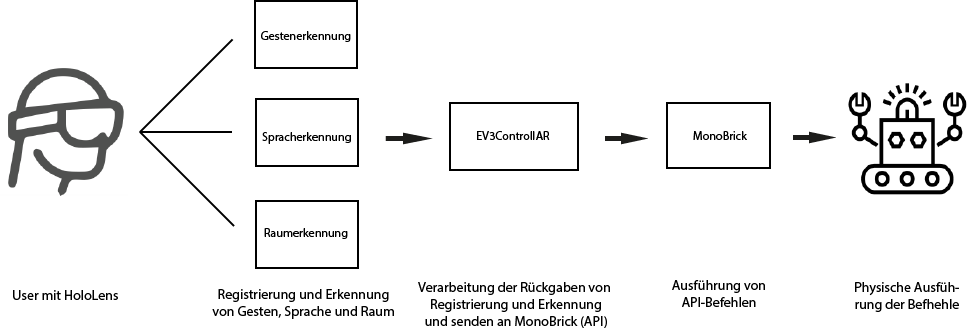
\includegraphics[width=1.0\textwidth]{figuren/Pipeline}
	\caption{Informationsfluss in der Applikation \textit{EV3ControllAR}. Bildquelle: Eigenes Werk.}
	\label{fig:pipeline}
\end{figure}
\subsection{Zielsetzung}
Das Ziel der Applikation ist es, zu erfassen, ob und inwieweit Gesten und Sprachkommandos eine natürliche Interaktionsform und Schnittstelle für die in Zukunft verschmelzenden Welten von Robotern und Menschen sind und ob Anwender diese beim Lösen kleiner Aufgaben als intuitiv empfinden.
\subsection{Anwendungsfall}\label{ssec:usecase}
Die funktionalen Anforderungen der Anwendung werden mit Hilfe von Anwendungsfällen ermittelt. Diese abstrahieren die Interaktion zwischen Benutzer und Anwendung und machen deutlich, was die Applikation aus Sicht des Benutzers leisten muss und inwiefern sie den Benutzer unterstützen kann. In Abbildung \ref{fig:useCaseDiagram} sieht man das Anwendungsfalldiagramm in der \textit{Unified Modelling Language}(UML) modelliert. Es zeigt die einzelnen Fälle der Applikation gebündelt in einem Diagramm. 
\begin{figure}[H]
	\centering
	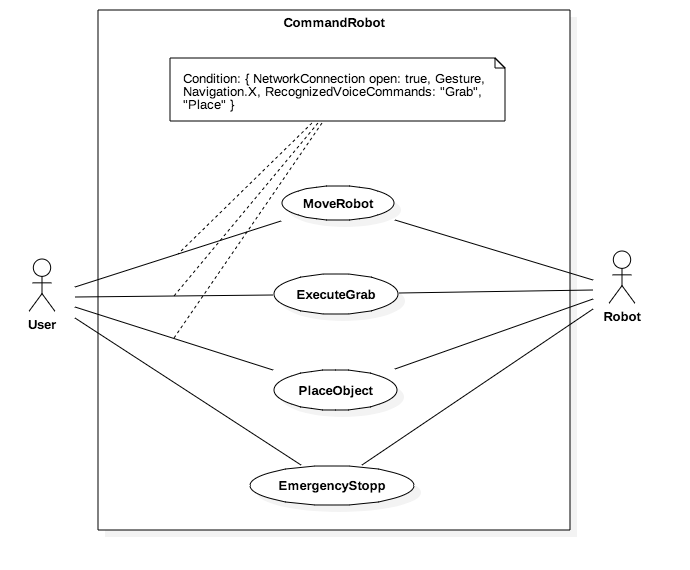
\includegraphics[width=1.0\textwidth]{figuren/UseCaseDiagram}
	\caption{UML \textit{Use-Case}-Diagramm -- CommandRobot. Bildquelle: Eigenes Werk.}
	\label{fig:useCaseDiagram}
\end{figure}
Aus diesem wurden dann drei explizitere untergeordnete Anwendungsfälle aufgegliedert. Diese wurden nach dem Prinzip der \textit{User Story} entwickelt. Die \textit{User Story} beschreibt aus Sicht des Anwenders oder Kundens, was eine Software leisten soll und was der Anwender sich diesbezüglich wünscht.\footnote{ Vgl. Wells, o.S., 1999, [Accessed: 04.01.2017].}

\textbf{Anwendungsfall 1 -- MoveRobot -- Roboter bewegen}\\
\frqq Als Anwender möchte ich den Roboter auf seiner Schiene frei bewegen können; dabei ist es mir wichtig, dass ich die volle Kontrolle über Geschwindigkeit und Position des Roboters habe.\flqq
\begin{table}[H]
	\centering
	\begin{tabular}{|l|p{8cm}|}
		\hline
		\textbf{Name} & Roboter bewegen (MoveRobot) \\
		\hline
		\textbf{Ziel im Kontext} & Roboter bewegt sich von Position A zu Position B \\
		\hline
		\textbf{Akteure} & Anwender und Roboter \\
		\hline
		\textbf{Trigger} & Anwender verschiebt 3D-Objekt in Szene \\
		\hline
		\textbf{Essentielle Schritte} & Richtiges 3D-Objekt auswählen \newline Korrekte Geste zum Translatieren in X-Richtung ausführen \newline 3D-Objekt freigeben \\
		\hline
		\textbf{Mögliche Erweiterungen} & Freies Translatieren ohne 3D-Objekt \\
		\hline
	\end{tabular}
	\caption{Anwendungsfall 1 -- \frqq Roboter bewegen\flqq.}
	\label{tab:usecase1}
\end{table}
\textbf{Anwendungsfall 2 -- GrabObject -- Objekt aufnehmen}\\
\frqq Als Anwender möchte ich mit Hilfe des Roboters Gegenstände in Reichweite aufheben; dabei ist es mir wichtig, dass der Roboter die Gegenstände präzise aufnimmt und bei Bewegungen in seinen Greifern behält.\flqq
\begin{table}[H]
	\centering
	\begin{tabular}{|l|p{8cm}|}
		\hline
		\textbf{Name} & Mit Roboter Objekt greifen (GrabObject) \\
		\hline
		\textbf{Ziel im Kontext} & Greift ein Objekt mit Greifern \\
		\hline
		\textbf{Akteure} & Anwender und Roboter \\
		\hline
		\textbf{Trigger} & Anwender verschiebt 3D-Objekt in Szene \\
		\hline
		\textbf{Essentielle Schritte} & Richtiges 3D-Objekt auswählen \newline Korrekte Geste zum Translatieren in Z-Richtung ausführen \newline 3D-Objekt freigeben \\
		\hline
		\textbf{Mögliche Erweiterungen} & Freies Translatieren ohne 3D-Objekt \\
		\hline
	\end{tabular}
	\caption{Anwendungsfall 2 -- \frqq Objekt aufnehmen\flqq.}
	\label{tab:usecase2}
\end{table}
\textbf{Anwendungsfall 3 -- PlaceObject -- Objekt platzieren}\\
\frqq Als Anwender möchte mit Hilfe des Roboters einen aufgenommenen Gegenstand an einer beliebigen Position ablegen; dabei ist es mir wichtig, dass der Roboter die Gegenstände präzise, druch öffnen der Greifer, absetzt und sie zur Aufnahme neuer Objekte offen hält.\flqq
\begin{table}[H]
	\centering
	\begin{tabular}{|l|p{8cm}|}
		\hline
		\textbf{Name} & Mit Roboter Objekt platzieren (PlaceObject)  \\
		\hline
		\textbf{Ziel im Kontext} & Roboterarm bewegt sich gen Boden und öffnet Greifer \\
		\hline
		\textbf{Akteure} & Anwender und Roboter \\
		\hline
		\textbf{Trigger} & Anwender aktiviert Sprachbefehl mit Stimme \\
		\hline
		\textbf{Essentielle Schritte} & Richtigen Sprachbefehl \newline Korrekte Abfolge von Worten aussprechen \newline \\
		\hline
		\textbf{Mögliche Erweiterungen} & Translatieren eines 3D-Objekts in Z-Richtung als Trigger \\
		\hline
	\end{tabular}
	\caption{Anwendungsfall 3 -- \frqq Objekt platzieren\flqq.}
	\label{tab:usecase3}
\end{table}
\textbf{Anwendungsfall 4 -- EmergencyStop -- Notstopp}\\
\frqq Als Anwender möchte ich den Roboter immer und mit sofortiger Wirkung anhalten können; dabei ist es mir wichtig, dass alle Motoren anhalten, Greifer und Arm sollten in ihrer bisherigen Position verweilen und der Bewegungsapparat zum Stehen kommen.\flqq
\begin{table}[H]
	\centering
	\begin{tabular}{|l|p{8cm}|}
		\hline
		\textbf{Name} & Notstopp (Stop)  \\
		\hline
		\textbf{Ziel im Kontext} & Roboter stoppt sofort alle Motoren \\
		\hline
		\textbf{Akteure} & Anwender und Roboter \\
		\hline
		\textbf{Trigger} & Anwender aktiviert Sprachbefehl mit Stimme \\
		\hline
		\textbf{Essentielle Schritte} & Richtigen Sprachbefehl oder \textit{Bloom}-Geste\\
		\hline
		\textbf{Mögliche Erweiterungen} & Notknopf am Körper. \\
		\hline
	\end{tabular}
	\caption{Anwendungsfall 4 -- \frqq Notstopp\flqq.}
	\label{tab:usecase4}
\end{table}
\subsection{Muss-Kriterien}
Die Anwendungsfälle resultieren in folgenden Funktionen, die dem Nutzer in der Applikation sofort und immer zur Verfügung stehen müssen:

\begin{itemize}
	\item Gestenerkennung
	\item Kenntlichmachung, wenn Gesten angewendet werden können (Gesture-Ready)
	\item Unterscheidung von Gesten:
	\begin{itemize}
		\item Tap-Geste um 3D-Objekte auszuwählen
		\item Tap-And-Hold-Geste um 3D-Objekte als \textit{draggable} auszuwählen
		\item Translatieren von 3D-Objekten in X-Richtung
	\end{itemize}
	\item Symbolisierung der oben genannten Gesten mit Icons
	\item Interface zur Übersicht des Roboters und dessen Funktionen
	\item \textbf{Notstopp}, sofortiger Stopp aller Motoren
\end{itemize}
\subsection{Kann-Kriterien}
Kann-Kriterien bezeichnen die Kriterien, deren Umsetzung sehr erstrebenswert wären. Allerdings sprengen sie im Kontext von Bachelorarbeiten meistens den zeitlichen Rahmen.

\begin{itemize}
	\item Roboter kann sich in allen Freiheitsgraden bewegen
	\item Dem Benutzer stehen weitere Gesten zur Verfügung
	\begin{itemize}
		\item Rotationsgesten, ähnlich dem Drehen eines Drehreglers
		\item \textit{Eyetracking} zur schnelleren Lokalisierung von Punkten im Raum
		\item Verbindung mit zusätzlichem \textit{Wearables} für mehr Interaktionsspielraum und Nutzung von bereits bekannten Gesten, wie \textit{Touch} oder Tasten
	\end{itemize}
	\item Roboter bewegt sich frei im Raum, nicht auf Schiene
	\begin{itemize}
		\item Wegfindung
		\item Visualisierung des Pfades im HMD
		\item Setzen von Wegpunkten aus dem HMD heraus
		\item Erweiterte Routenoptionen
	\end{itemize}
	\item Weitere Anwendungsszenarien
\end{itemize}
\subsection{Abgrenzungskriterien}
Die Abgrenzungskriterien stellen Kriterien dar, welche aufzeigen, was das System nicht leisten soll, um es klar von anderen Systemen abzugrenzen.

Die Grenzen dieses Produkts belaufen sich im Allgemeinen darauf, dass die Applikation nur ein Prototyp ist, welcher die Machbarkeit überprüfen und das Gefühl der kontrollierten Steuerung übertragen soll. Sie belaufen sich des Weiteren auf folgende Punkte:
\begin{itemize}
	\item Verwendbarkeit unter echten Produktionsbedingungen
	\item Verwendung in Echtzeit
	\item Synchronität von Gesten und Bewegung des Roboters
	\item Sicherheit
	\item Skalierbarkeit
	\item Simultane Verwendbarkeit eines Roboters durch mehrere Anwender
	\item Generische Nutzung von Maschinen
\end{itemize}
\subsection{Nicht funktionale Kriterien}
Was \frqq nicht funktionale Kriterien\flqq\ sind, ist nicht einheitlich definiert, jedoch ist allen Definitionen gemein, dass \frqq nicht funktionale Kriterien\flqq\ mit Metriken beschreiben, wie gut/zuverlässig ein System funktionieren soll.\footnote{ Vgl. Rupp, S. 268f, 2014.}\\
In der vorliegenden Arbeit wird besonderer Wert darauf gelegt, dass die Applikation \textit{EV3ControllAR} folgende Kriterien erfüllt:
\paragraph*{Aussehen}
Ebenso ist es für die Anwendung der vorliegenden Arbeit wichtig, dass sowohl das \textit{Interface} Design als auch die Code-Struktur sauber, modern, übersichtlich und gut strukturiert ist. Dazu zählt auch die Wartbarkeit des Codes durch Lesbarkeit und fundierte Dokumentation.
\paragraph*{Benutzbarkeit}
In der vorliegenden Arbeit wird ebenfalls hoher Wert darauf gelegt, dass die Anwendung eine leichte Verständlichkeit bietet, sodass sich dem Anwender die Benutzbarkeit erschließt und durch er visuelle Signale gestützt wird. Außerdem sollte sie, soweit dies bei innovativen Interaktionsformen möglich ist, durch sich wiederholende, bekannte und bereits erlernte Muster und Metaphern gefördert werden. Hinzu kommt die Reaktionszeit des Roboters, die unter einer Sekunde liegen soll.
\subsection{Anwendungsumgebung}
In diesem Bereich wird erläutert, in welcher Anwendungsumgebung die Applikation ihren Sinn findet und unter welchen Bedingungen sie läuft. Zunächst sei dargelegt, dass die prototypische Version nur unter Laborbedingungen arbeitet, wohingegen das Konzept sowohl für Werkshallen, als auch menschenfeindliche Arbeitsumgebungen,
beispielsweise die Atmosphäre eines anderen Planeten, verseuchte oder unwegsame
Gebiete der Erde, das All oder auch alle Umgebungen, bei denen ein ferngesteuerter Roboter einen Sinn ergibt, entwickelt wurde.

Die Anwendung an sich kann dank \textit{Unity} für verschiedene Betriebssysteme kompiliert werden. Allerdings macht es nur Sinn, sie als Windows-App für die \textit{HoloLens} zu \textit{builden}, da die Schnittstellen des \textit{HoloToolkit} nur die Datenbrille von Windows ansprechen. Für die Ausführung unter Laborbedingungen benötigt man folgende Hardware:
\begin{itemize}
	\item \textit{Microsoft HoloLens}
	\item \textit{Lego Mindstorms EV3} mit \textit{WiFi USB-Dongle}
	\item Roboterarm aus \textit{Lego}
	\begin{itemize}
		\item MotorA - Translation im Raum
		\item MotorB - Rotation um Armgelenk
		\item MotorC - Greifer auf/zu
		\item Führungsschiene für den Roboter
		\item Objekt, das bewegt werden soll
	\end{itemize}
	\item Router für ein lokales Netzwerk
\end{itemize}
Der Softwareteil beschränkt sich auf die Applikation \textit{EV3ControllAR}.
\begin{itemize}
	\item Client Applikation auf HoloLens
\end{itemize}
Abbildung~\ref{fig:ev3_robot} zeigt den Versuchsaufbau für die prototypische Implementierung.
\begin{figure}[H]
	\centering
	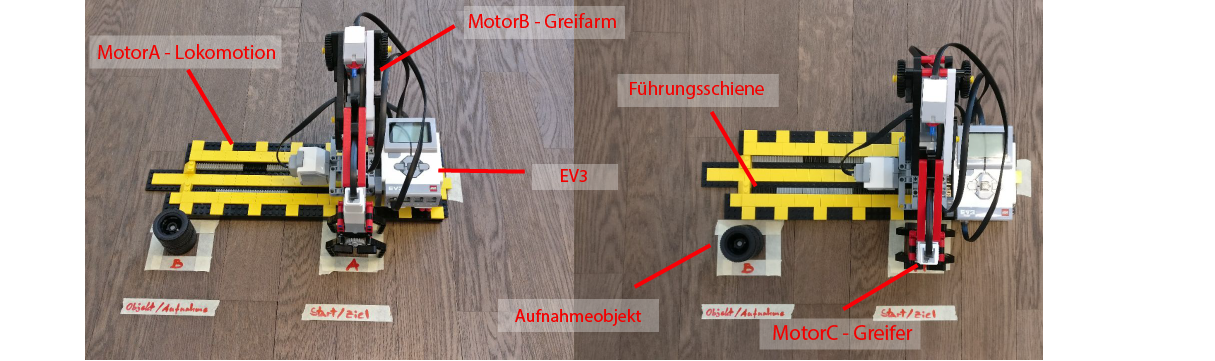
\includegraphics[width=1.0\textwidth]{figuren/ev3_robot}
	\caption{Versuchsaufbau für die Applikation \textit{EV3ControllAR}. Bildquelle: Eigenes Werk.}
	\label{fig:ev3_robot}
\end{figure}
%
%Außerdem entfallen außer der Netzwerkverbindung, der HoloLens und dem Roboter selbst alle Laborbedingungen.
\subsection{Anwendungsdaten}
Dieser Abschnitt beschäftigt sich mit den Daten, die vom Anwender ins System eingepflegt werden müssen. Auch hier wird wieder zwischen Prototyp und Konzept unterschieden. So muss ein User beim Prototyp keine spezifischen Produktdaten eingeben. Allerdings ist es von höchster Priorität, dass ein Maschinenführer sich bei wertvollem Baustellenequipment und schweren Baumaschinen zur Nutzung autorisiert. Heutzutage läuft dieser Prozess meistens noch wie folgt ab: Eine Autorisierung erfolgt über optionale Schlüsselqualifikationen, wie beispielsweise einem Baggerführerschein, Staplerführerschein oder Drohnenführerschein. Die Scheine sind meistens kein \frqq Muss\flqq, begünstigen allerdings den Eindruck und die versicherungsspezifischen Bedingungen des Arbeiters. Die Scheine werden in Schulungen erworben. Die Qualifikation wird beim Arbeitgeber vorgelegt, welcher dann den Arbeiter zum Maschinenführer ernennt und ihm einen Schlüssel aushändigt, der den Arbeiter zum Starten der Maschine befähigt. Eine Schulung, wie oben beschrieben, soll es auch für virtuelle Interaktion geben. Im ausgeführten Thinkaloud-Test bekommen die Probanden beispielsweise eine Einführung in die Interaktionen. Allerdings könnte die Autorisierung an der Maschine über Stimme, Fingerabdruck, Iris-Scan oder andere innovative Authentifizikationsmechanismen stattfinden.
\subsection{Anwendungsszenario}\label{ssec:applicationScenario}
Dieser Abschnitt beschäftigt sich mit dem Anwendungsszenario der prototypischen Implementierung, aber auch mit konzeptionellen Erweiterungen.

Das Szenario hat als Hauptaufgabe, die Anwendung in den Kontext der Mensch-Maschine-Interaktion zu setzen. Deswegen bekommen die Testprobanden Hilfestellung in Form eines Tutoriums, welches die Gesten erklärt, und danach folgende Aufgabe, die es zu bewältigen gilt:
\paragraph*{Aufgabenstellung an die Testprobanden}
\begin{enumerate}
	\item Orientieren Sie sich in der Szene mit Hilfe des Cursors und zeigen Sie mit diesem auf das Steuerelement.
	\item Heben Sie eine Hand und bringen Sie sie in die \textit{Gesture-Ready}-Position.
	\item Bewegen Sie nun den Roboter mit Hilfe des Interaktionselements und der \textit{Tap-And-Hold}- und \textit{Translation}-Geste von Position A zum Aufnahmeort des Objektes.
	\item Am Objekt angekommen aktivieren Sie über den Sprachbefehl \frqq GRAB\flqq\ die Aufnahme des Objekts durch den Roboterarm.
	\item Bewegen Sie den Roboterarm nun zurück zu Position A.
	\item Dort angekommen setzen Sie das Objekt ab, indem Sie den Sprachbefehl \frqq PLACE\flqq\ aussprechen.
\end{enumerate}
Weitere mögliche Szenarien sind, dass Anwender versuchen Objekte zu
stapeln oder zu sortieren. Außerdem könnte man erproben, das Objekt während der
Fahrt aufzunehmen oder abzusetzen. Verändert man die Führungsschiene des Roboters oder gibt ihm einen anderen Antriebsmodus, wie Räder oder Ketten, kann man den Prototyp auch unter freieren Bedingungen testen. Tests im Gelände und Ferntests sind aus Sicht des Autors der nächste logische Schritt.
\section{Systementwurf und entwicklungsspezifische Technologien}
Diese Sektion gibt in erster Linie Einblicke in die grundlegende Interaktion mit dem System. Dazu werden die wichtigsten Funktionalitäten anhand von \textit{Wireframes} und Systementwürfen erläutert. Im Anschluss folgt eine Einführung in die verwendeten Technologien und Bibliotheken. Der Teil dieser Applikation, der sich mit der Benutzerseite beschäftigt, ist stark von Interaktion und visuellen Reizen geprägt. Wie soll beispielsweise deutlich gemacht werden, welches Szenenobjekt wann bewegt werden soll und welche Möglichkeiten der Interaktion es gibt?
\subsection{Unity 5.5f}
Diese Sektion beschäftigt sich mit der \textit{Game Engine Unity}5.5f und mit ihrer Beschaffenheit, sowie damit, welche Vorteile \textit{Unity} bietet und weshalb die genannte Version gewählt wurde.\paragraph*{Unity}  \frqq ist eine Laufzeit- und Entwicklungsumgebung für Spiele (Spiel-Engine) des Unternehmens Unity Technologies mit Hauptsitz in San Francisco\flqq.\footnote{ Wikipedia, Unity (Spiel-Engine), [Accessed: 14.02.2017].} Das Unterstützen von Multiplattform-Kompilierung (siehe Abbildung \ref{fig:unity_builds}) und einer breit gefächerten Entwickler- und Unterstützergemeinschaft verhalf \textit{Unity} in den letzten Jahren dazu, die beliebteste Spiele-Engine der Welt zu werden.\footnote{ Unity - Anonymous, Unternehmensfakten, 2016, [Accessed: 14.02.2017].}
\begin{figure}[H]
	\centering
	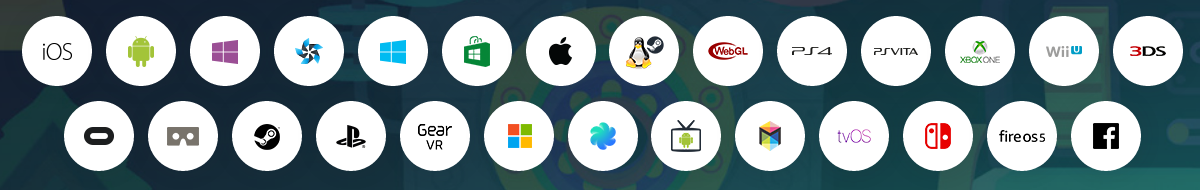
\includegraphics[width=1.0\textwidth]{figuren/unity_builds}
	\caption{\textit{Unity} Multiplattform-Unterstützung -- Übersicht der unterstützten Plattformen. Bildquelle: \cite{unity}.}
	\label{fig:unity_builds}
\end{figure}
\paragraph*{Entwicklungsumgebung}
Die Hauptansicht von \textit{Unity}, der \textit{Editor}, beinhaltet die Unterfenster \textit{Scene}, in der die 3D-Szene durch \textit{GameObjects} manipuliert werden kann; diese \textit{GameObjects} werden in einem Szenengraph organisiert, der im Panel \textit{Hierachy} dargestellt wird und dessen Attribute wiederum im Panel \textit{Inspector} angezeigt werden und dort auch verändert werden können. Sie werden mit \textit{Components} bestückt, um ihnen bestimmte Funktionen zu geben. Sobald der \textit{Play-Button} aktiviert wurde, zeigt das Fenster \textit{Game} das Spiel aus der Sicht der aktiven Kamera. Man nutzt dieses zum Testen seiner Applikation, es ermöglicht schnelle Iterationszyklen, da das Programm nicht nach jeder Änderung kompiliert und auf das Zielgerät übertragen werden muss. In Abbildung \ref{fig:unity_editor} sieht man ein solches Unity-Editor-Fenster und seine Panele auf einen Blick. Mit dem \textit{Scene}- und \textit{Hierachy}-Fenster lassen sich durch bereits vorgefertigte \textit{Components} und viele, von anderen Leuten bereits angefertige \textit{Assets} aus dem \textit{Assetstore}, auf Anhieb kleinere Spiele, auch ohne Programmierkenntnisse, fertigen.
\begin{figure}[H]
	\centering
	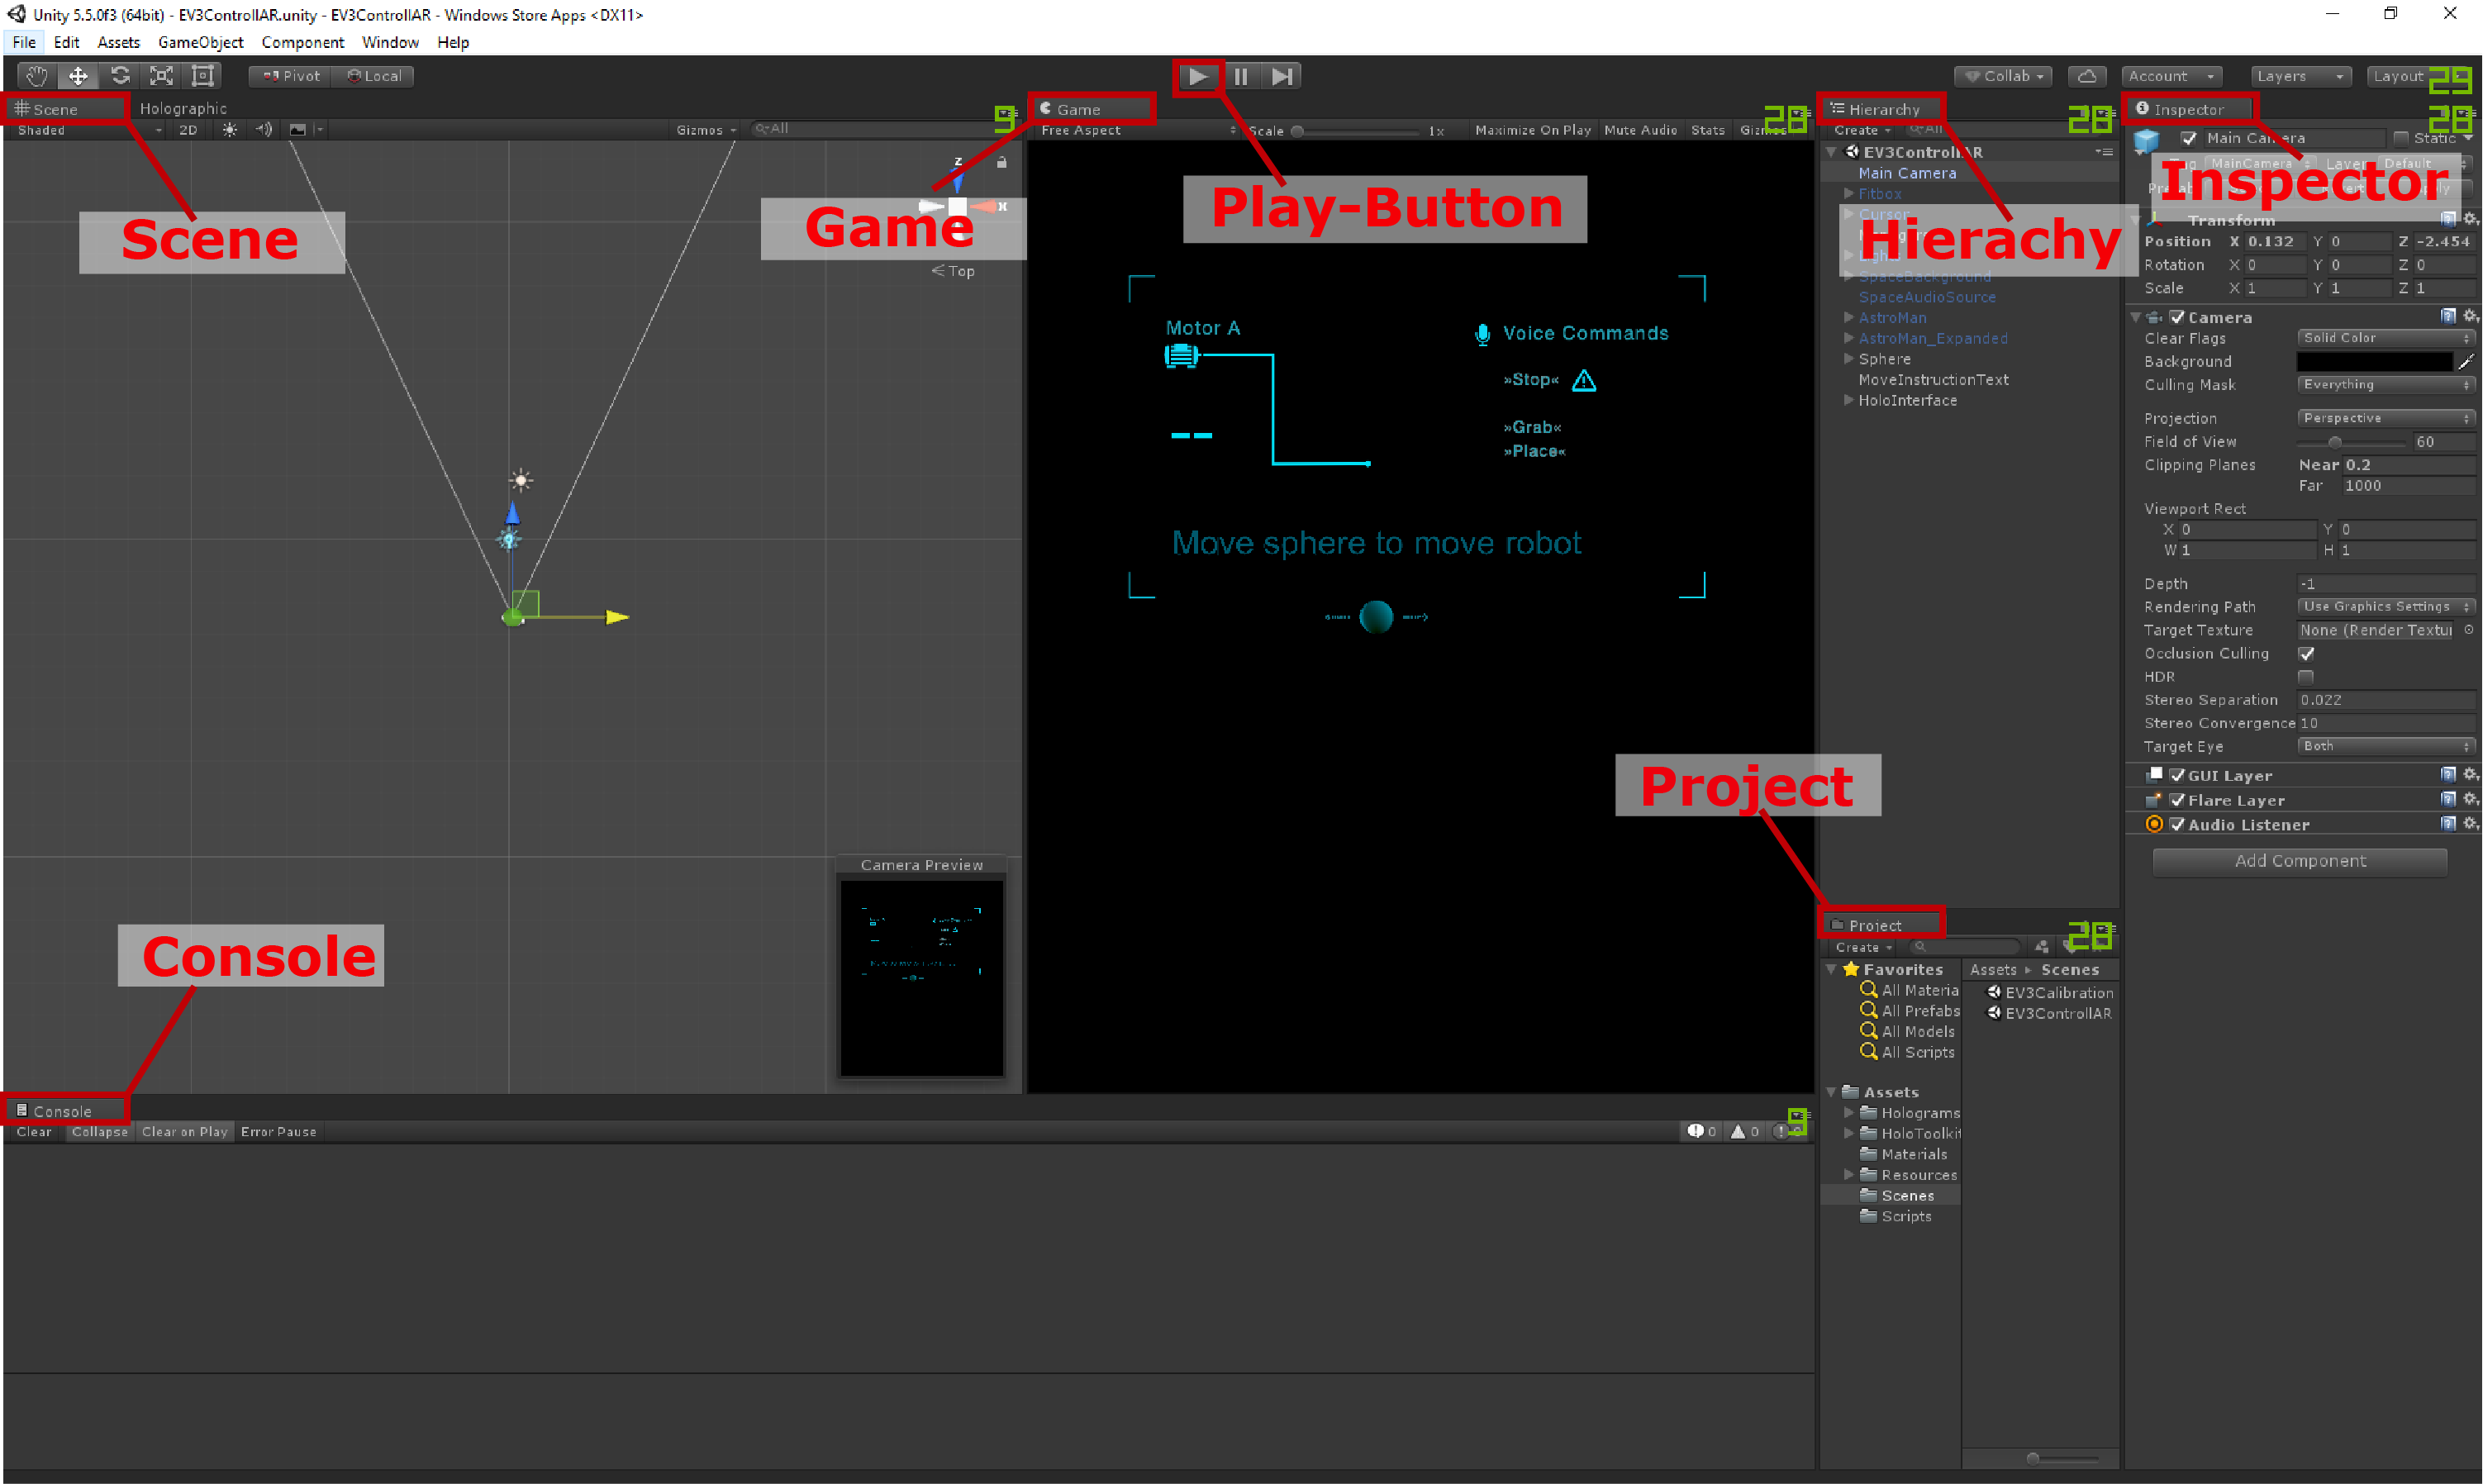
\includegraphics[width=1.0\textwidth]{figuren/Unity_Editor}
	\caption{\textit{Unity} Entwicklungsumgebung -- Übersicht des Editors. Bildquelle: Eigenes Werk.}
	\label{fig:unity_editor}
\end{figure}
\paragraph*{Skripts}
Möchte man allerdings seiner Applikation mehr Funktionalität geben, tut man dies durch das Anhängen eigener \textit{Scripts} als \textit{Component} an die \textit{GameObjects}. Die Skriptsprache ist \textit{C\#} oder \textit{Unity-Script}, welches an JavaScript angelehnt ist. Der \textit{Inspector} von Unity interagiert mit den Variablen aus den Skripten. Deklariert man beispielsweise eine Variable mit der Zugriffsklasse \textit{public} wird diese im \textit{Inspector} angezeigt und man kann sie direkt aus \textit{Unity} per \textit{Drag and Drop} initialisieren.
\paragraph*{Grafik}
\textit{Unity}s Grafikpipeline bedient die \textit{Rendering}-Pfade:
\begin{itemize}
	\item \textit{Forward Rendering}
	\item \textit{Deferred Shading}
	\item \textit{Legacy Deferred Lightning}
	\item \textit{Legacy Vertex Lit}
	\item \textit{Shadows}
\end{itemize}

\textit{Shader}, welche in der \textit{High-Level-Shader-Language}(HLSL) geschrieben werden, bestimmen wie Objekte in der Szene aussehen, indem sie die Materialeigenschaften und die Beleuchtung dazu berechnen.\footnote{ Unity, Rendering Pipeline \url{https://docs.unity3d.com/Manual/SL-RenderPipeline.html}.}

Das besondere an der Version 5.5f ist, dass sie \textit{HoloLens Ready} ist. In ihr wurden die Versionen \textit{Unity 5.4.0f3-HTP}, was für den Entwicklungszweig die \textit{HoloLens} betreffend steht, sowie der ursprüngliche Entwicklungspfad von \textit{Unity} zusammengeführt und zusätzliche Zusatzfunktionen implementiert, die das Entwickeln mit und für die \textit{HoloLens} erheblich vereinfachen und beschleunigen. Dazu zählen beispielsweise das Starten des entwickelten Projekts direkt aus dem \textit{Editor}, was die Iterationszyklen, gegenüber dem Kompilieren und Übertragen des Programms per \textit{USB} oder \textit{WiFi} auf die \textit{HoloLens}, erheblich beschleunigt, sowie das Bereitstellen von Funktionalitäten des \textit{HoloToolkit}, welches in der folgenden Sektion~\ref{ssec:HoloToolkit} genauer betrachtet wird.
\subsection{HoloToolkit}\label{ssec:HoloToolkit}
Das \textit{HoloToolkit} ist \frqq eine Kollektion von Skripten und Komponenten, welche beabsichtigt die Entwicklung von holografischen Applikationen für \textit{Windows Holographics} zu beschleunigen.\flqq\footnote{ Microsoft, HoloToolkit Repository, 2016, [Accessed: 15.02.2017].} Das \textit{Toolkit} beinhaltet viele nützliche Schnittstellen\footnote{ Microsoft, HoloToolkit Repository, 2016, [Accessed: 15.02.2017].} für die \textit{HoloLens}, grob gegliedert in: 
\begin{enumerate}
	\item Input
	\item Sharing
	\item Spatial Mapping
	\item Spatial Understanding
	\item Spatial Sound
	\item Utilities
	\item Build
\end{enumerate}
Die vorliegende Arbeit beschäftigt sich und nutzt hauptsächlich die Inhalte der Sektion \textit{Input}, im folgenden Abschnitt werden seine Bestandteile genauer betrachtet.
\paragraph*{Input}
Das \textit{Input}-System beinhaltet ein voll funktionsfähiges Eingabe-Modul, dies erlaubt dank einer Implementation basierend auf Schnittstellen ein erweiterbares Modul, welches die Hauptcharakteristiken \textit{Gaze}, \textit{Gesture} und \textit{Voice} abdeckt. Es liefert vorgefertigte Objekte und Skripte mit, die zum einen dafür sorgen, dass Grundfunktionen wie \textit{Gaze} immer gleich, beziehungsweise ähnlich implementiert werden und zum anderen die Entwicklung beschleunigen.
\subsection{MonoBrick API}\label{ssec:monoBrick}
Die \textit{MonoBrick API} ist ein Paket, das aus der \textit{MonoBrick EV3 Firmware} entstanden ist, welche es erlaubt den \textit{EV3} mit dem \textit{opensource .Net Framework} namens {Mono} programmiert und \textit{debuggt} werden kann.\footnote{ Vgl. Soborg / Jeppesen, o.J., [Accessed: 22.02.2017].} Sie wurde von Anders Soborg und Lars Jeppesen entwickelt und macht sie für ein \textit{Unity}-Projekt besonders wertvoll, da durch die \textit{.Net}-Umgebung in \textit{C\#} entwickelt werden kann. Die Schnittstelle \textit{MonoBrick Communication Library} agiert dabei als \textit{Wrapper} für die \textit{LEGO Mindstorms Communication Library} in \textit{C\#}, welche mit der Standard-\textit{Firmware} des \textit{EV3} funktioniert. Allerdings musste für die Nutzung mit \textit{Unity} die Bibliothek zunächst herunterkompiliert werden, da \textit{Unity} momentan nur die \textit{.Net 2.0}-Umgebung unterstützt, die \textit{MonoBrick Communication Library} allerdings für die \textit{.Net 4.0}-Umgebung entwickelt wurde. Die Entwicklungsumgebung \textit{Microsoft Visual Studio 2015 professional} lässt ein solches Abstufen von \textit{.dll} Paketen zu und unterstützt den Entwickler dahingehend im \textit{Build}-Menü ein Ziel-\textit{Framework} auszuwählen.